\chapter{理論}
\section{イオントラップ}
電荷を持つイオンは電場によって力を受けることから,電磁場を用いることで空間に閉じ込めることが可能になっている.これを可能にする装置をイオントラップと呼ぶ.電磁気学において,アーンショーの定理と呼ばれる定理が知られており,この定理によれば静電ポテンシャルを記述するラプラス方程式の解に極大値および極小値が表れない.つまり,静電場のみを用いてイオンを捕獲することが不可能になっている.イオンを閉じ込めるためには,静電場と静磁場を使ったペニンブトラップ,あるいはrf(radio frequency)電場と静電場を用いたパウルトラップが主に使用される.本研究では後者のパウルトラップの原理を応用させた平面型のイオントラップ.プレーナートラップを使用してイオンの捕獲を行っていることから,パウルトラップについて述べる.
\section{パウルトラップ}
\subsection{rf擬ポテンシャル}
\large
\begin{align}
	\Phi_{\rm eff}(x,y,z) = \frac{e^2}{4m\Omega_{\rm rf}^2}|\vec{E}(x,y,z)|^2
\end{align}
\normalsize
\subsection{イオンの運動}
Mathieu方程式
\large
\begin{align}
	\frac{{\rm d^2}r_i}{{\rm d}t^2} + [a_i + 2q_i \cos (\Omega_{\rm rf} t)]\frac{\Omega_{\rm rf}^2}{4}r_i = 0. \quad (i = x,y,z)
\end{align}
\normalsize
\subsection{余剰マイクロ運動}
浮遊電場が存在する場合のMathieu方程式
\large
\begin{align}
	\frac{{\rm d^2}r_i}{{\rm d}t^2} + [a_i + 2q_i \cos (\Omega_{\rm rf} t)]\frac{\Omega_{\rm rf}^2}{4}r_i = \frac{e\vec{E}_{\rm stray}\cdot \hat{r}_i}{m}. \quad (i = x,y,z)
\end{align}
\normalsize
rfに起因,レーザーによって冷却することができない
\section{プレーナー型パウルトラップ}
\begin{figure}[h]
	\begin{center}
		\begin{minipage}{0.48\linewidth}
			\begin{center}
			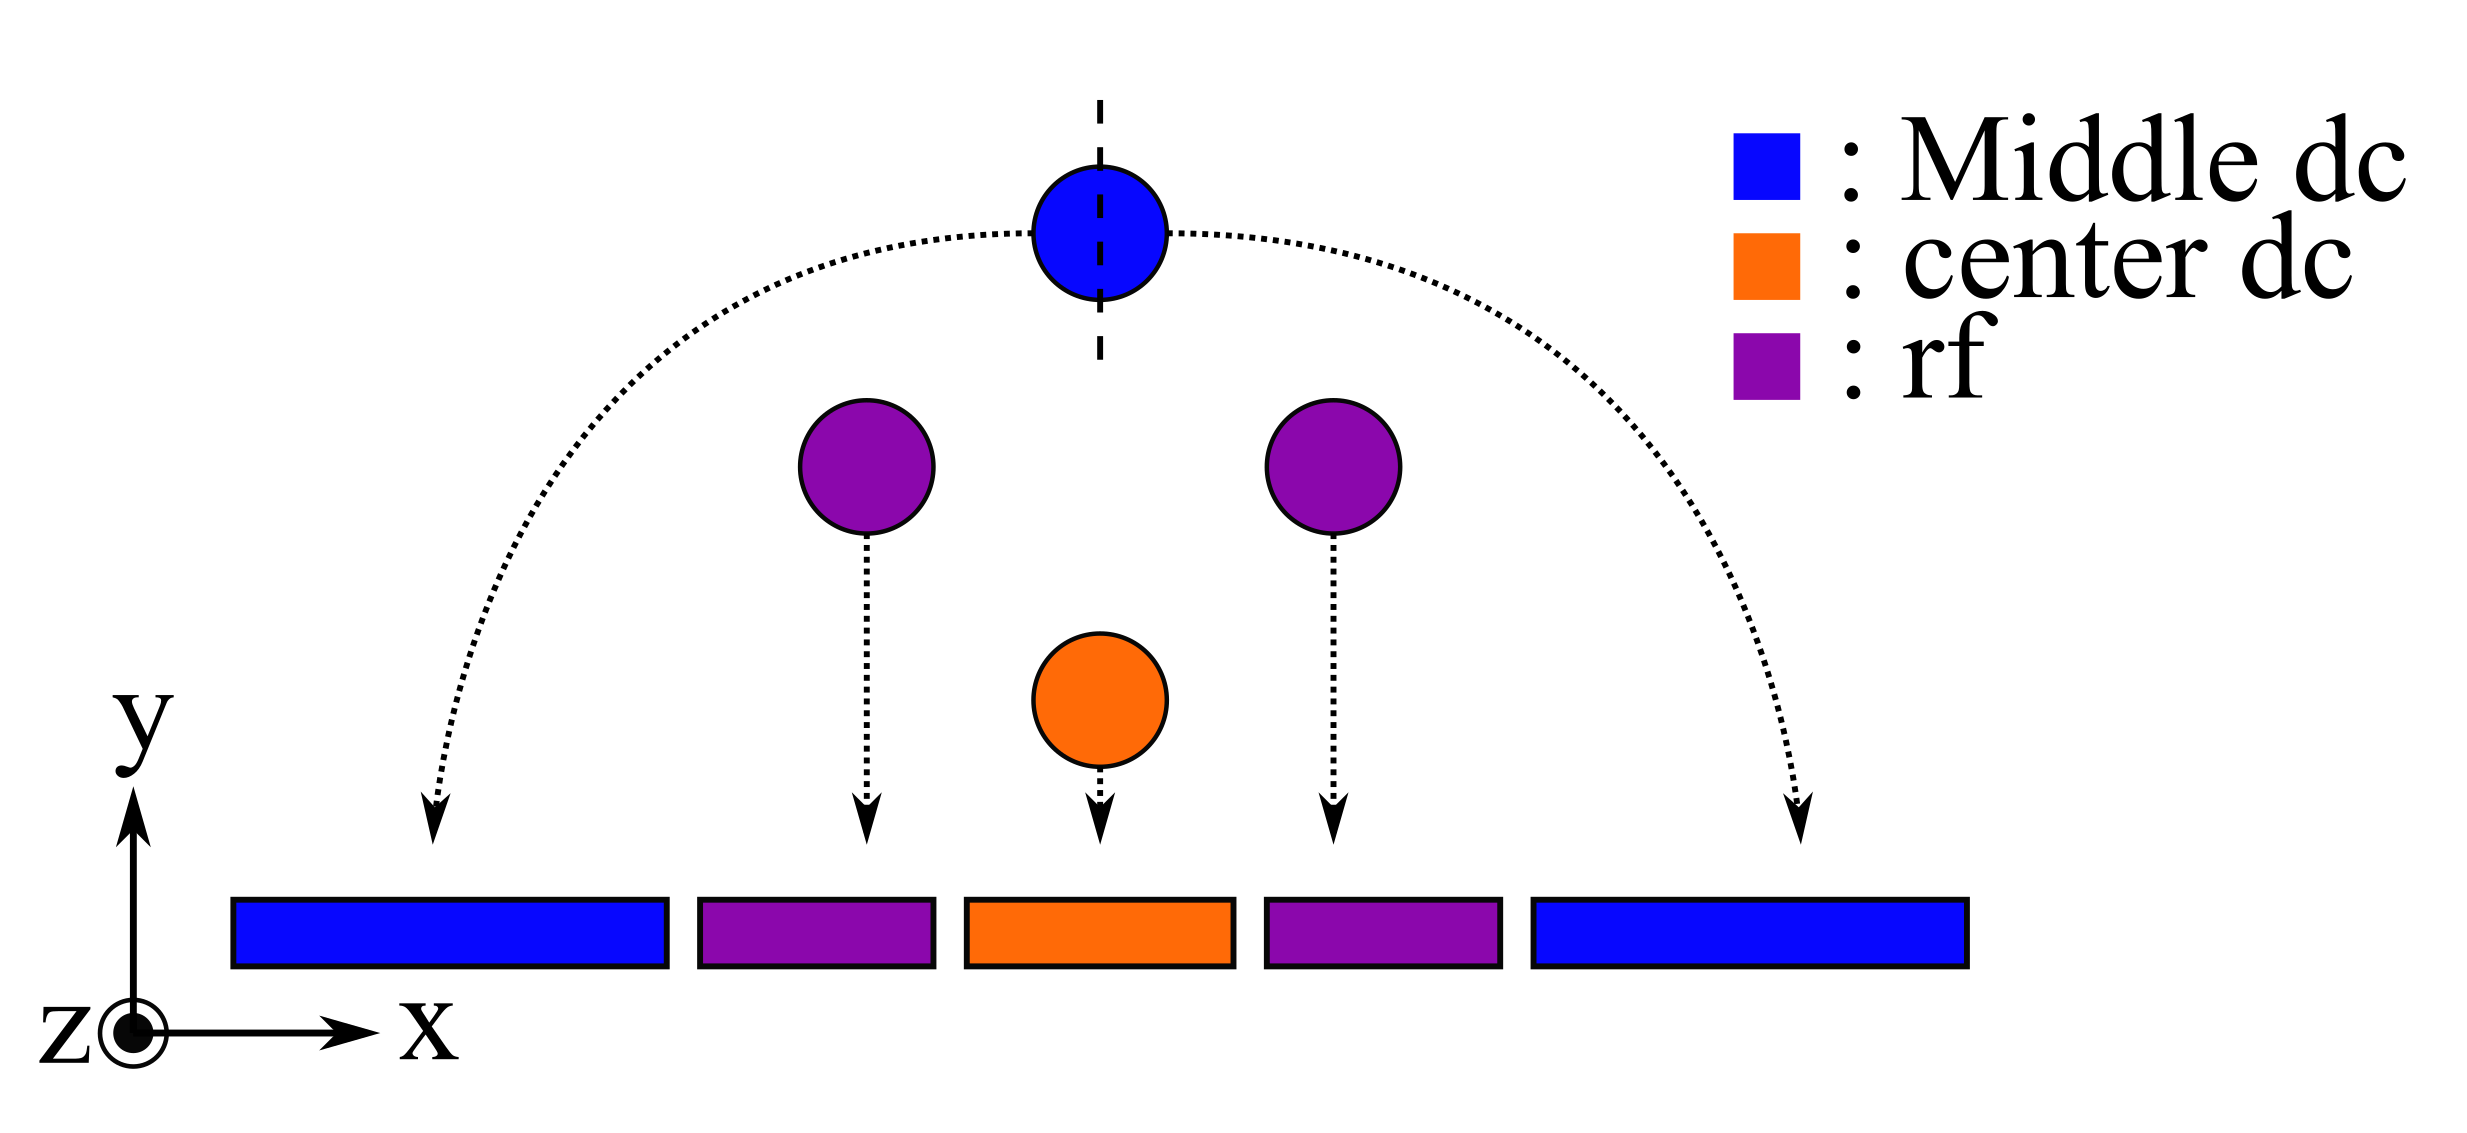
\includegraphics[width = 0.98\columnwidth]{./theory/figure/PaulTrap_3Dto2D_3DTrap.png}
			\end{center}
		\end{minipage}
		\begin{minipage}{0.48\linewidth}
			\begin{center}
			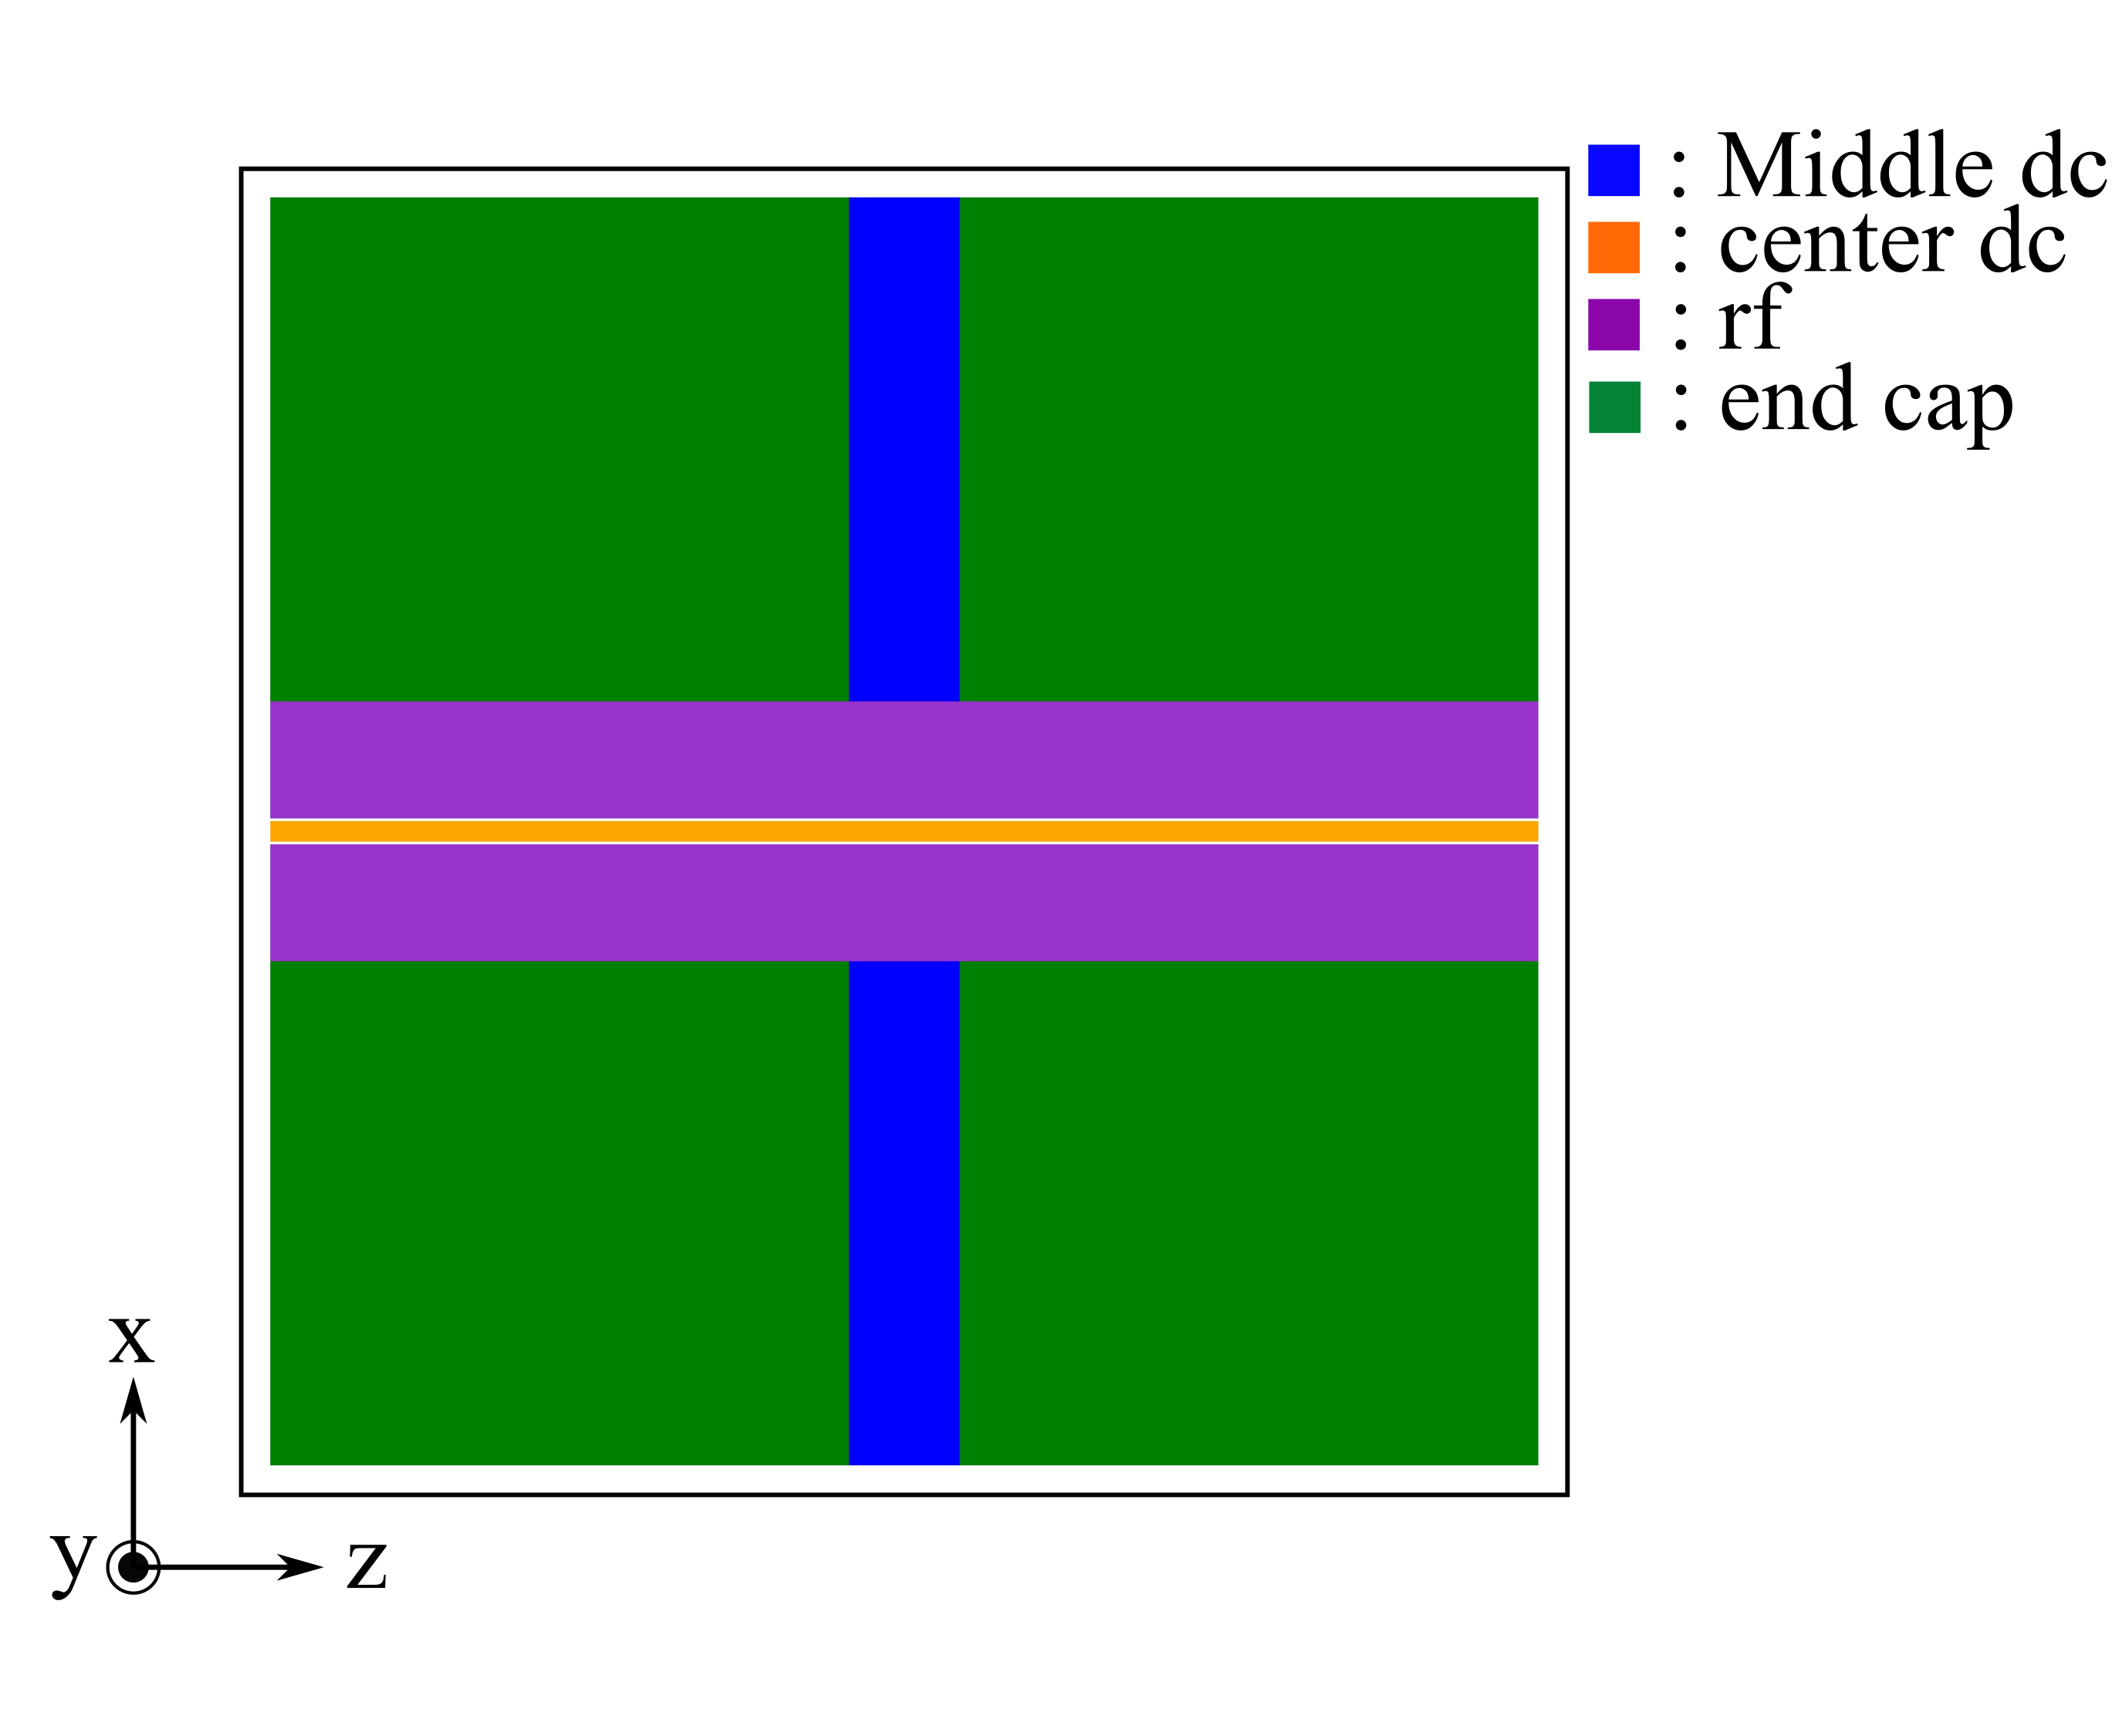
\includegraphics[width = 0.98\columnwidth]{./theory/figure/PaulTrap_3Dto2D_2DTrap.png}
			\end{center}
		\end{minipage}
	\end{center}
	\caption{立体的なパウルトラップとプレーナー型パウルトラップとの対応関係}
\end{figure}
\subsection{電極の仕様}
\begin{figure}[h]
	\begin{center}
		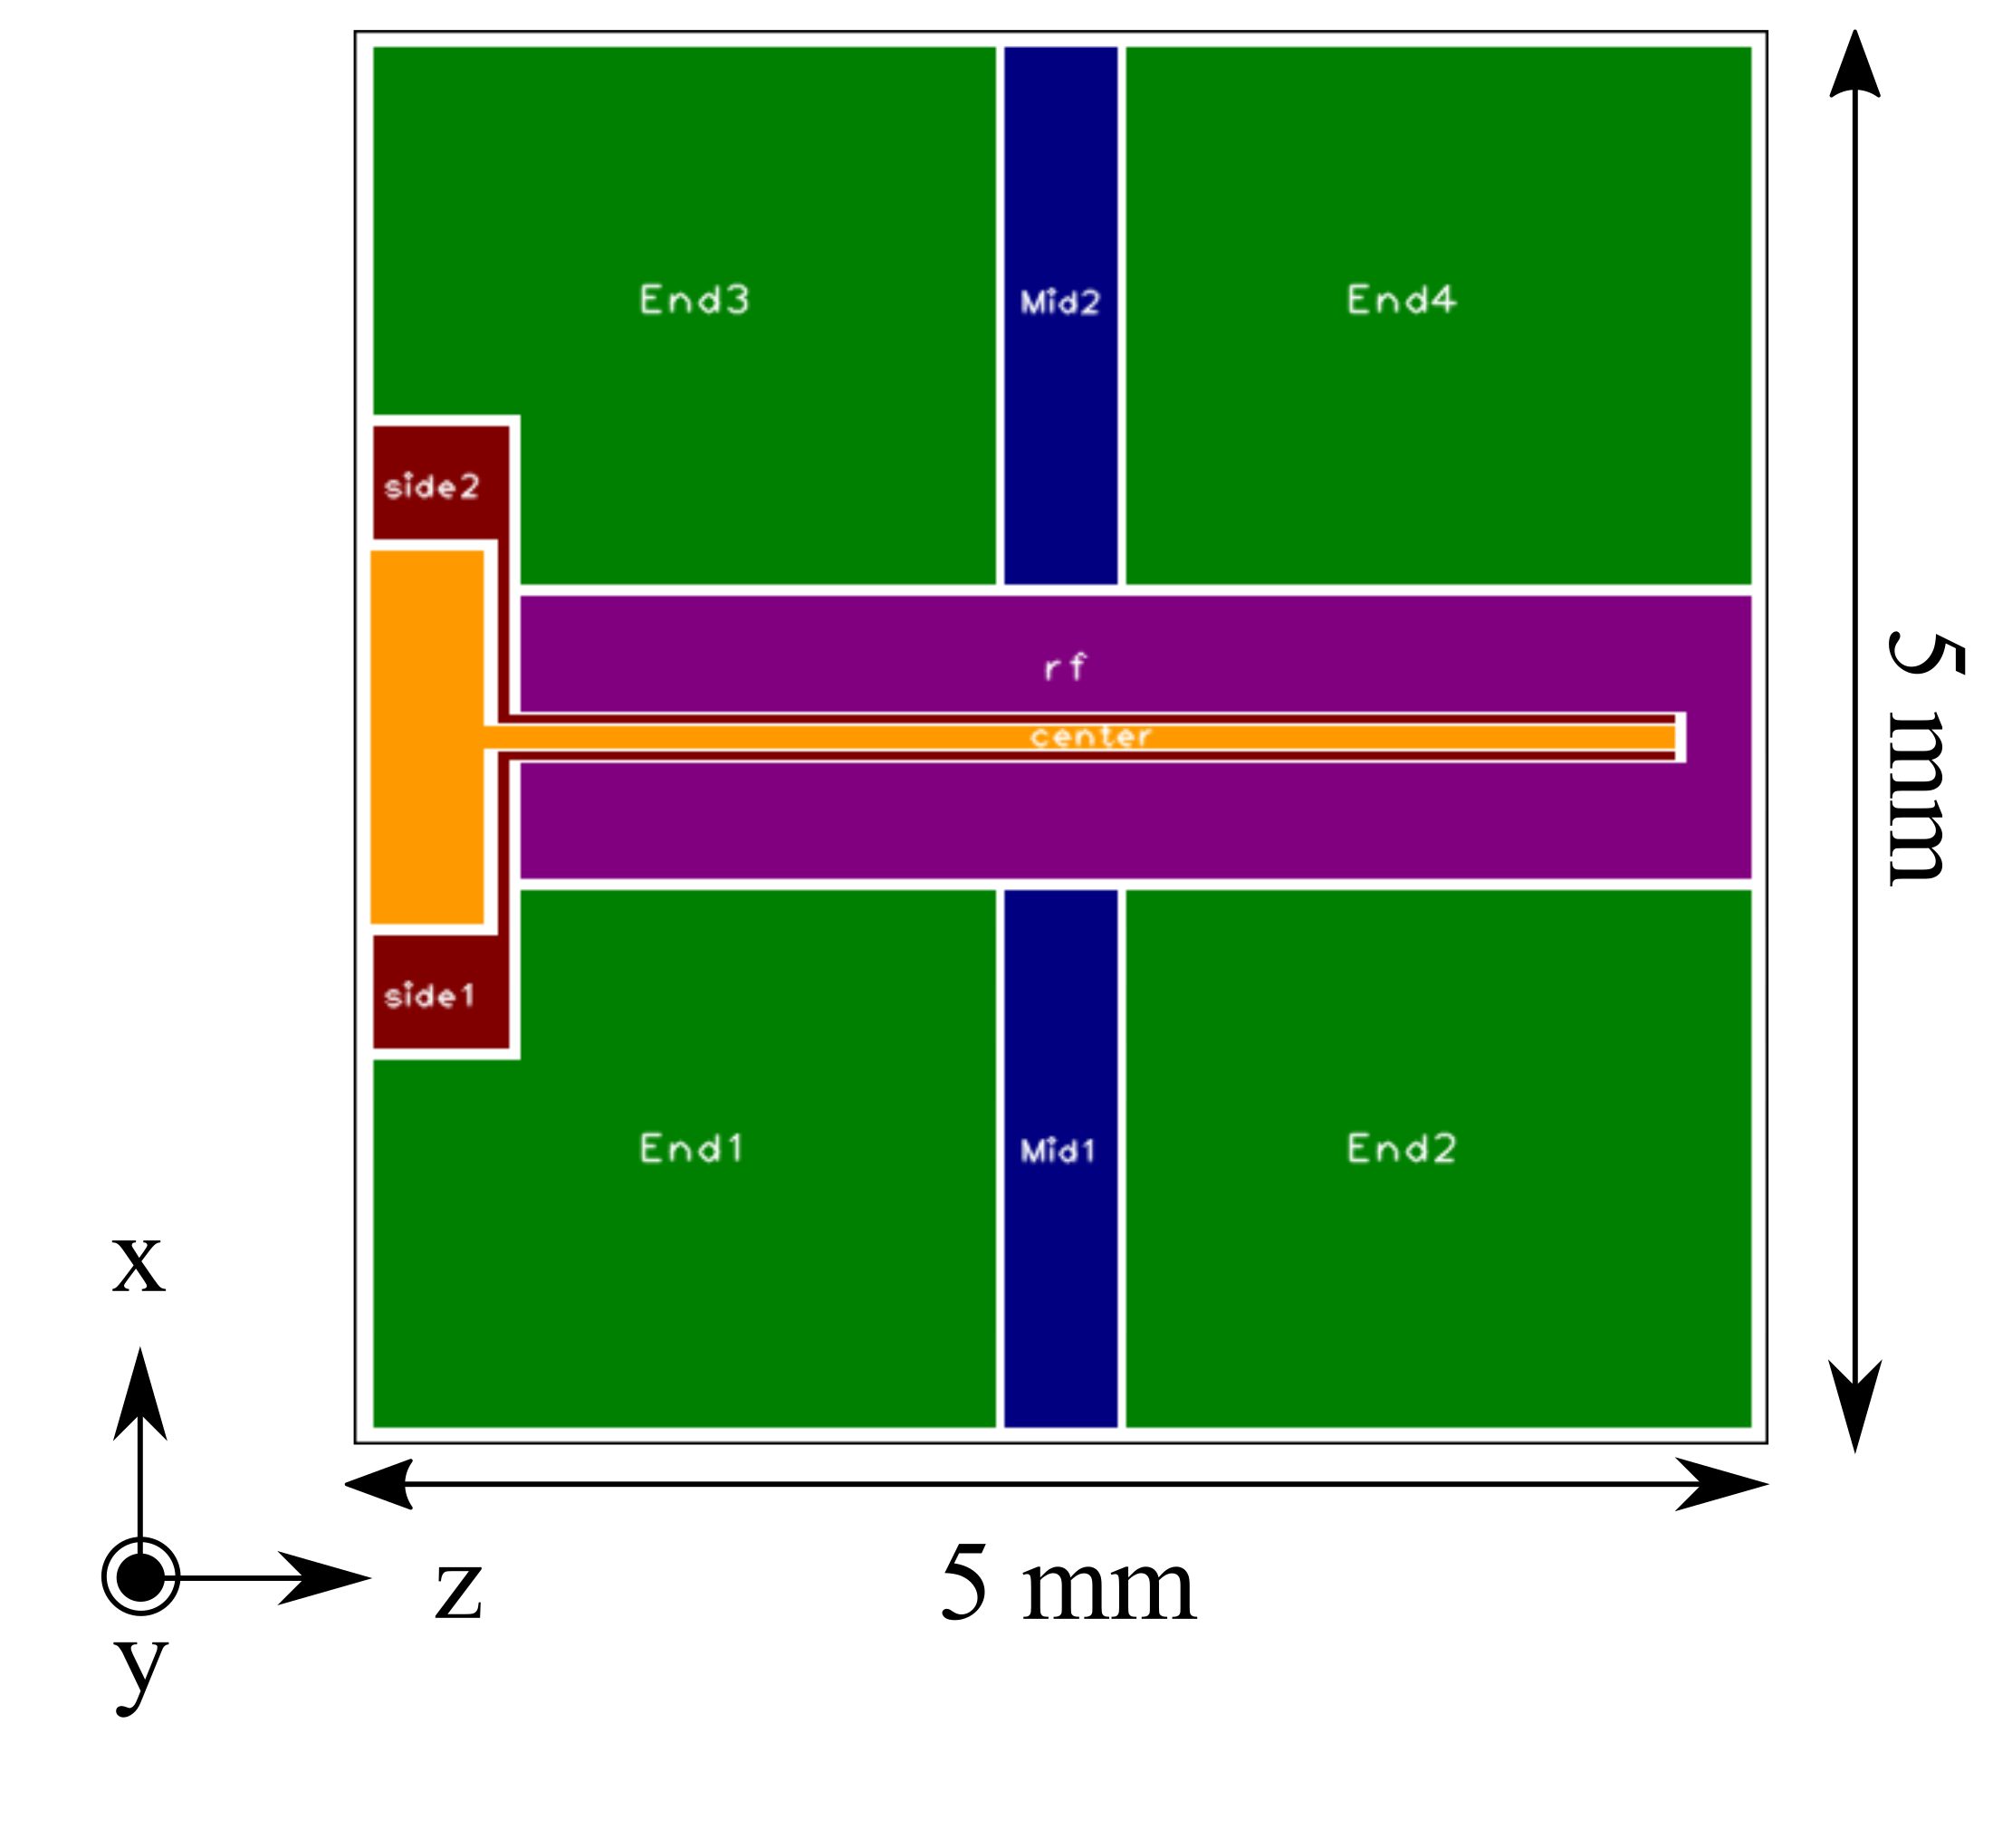
\includegraphics[width = 0.5\linewidth]{./theory/figure/named_electrode.png}
		\caption{本実験で使用するプレーナー型パウルトラップの電極モデル}
		\label{fig:Named_PlannerTrap}
	\end{center}
\end{figure}
以下では,プレーナー型パウルトラップのことを単にプレーナートラップと呼ぶ.
\subsection{矩形電極が作る静電ポテンシャル}
\begin{figure}[h]
	\begin{center}
		
\includegraphics[width = 0.5\linewidth]{./theory/figure/Potential_of_rect-electrode.png}
		\caption{$(z_1,x_1),(z_2,x_2)$で指定される矩形が任意の点$(x,y,z)$に形成する静電ポテンシャル}
		\label{fig:Potential_from_rect-electrode}
	\end{center}
\end{figure}
\begin{align}\label{eq:rectangle_electrode}
	\phi(x,y,z) = \frac{V}{2\pi} \left\lbrace \arctan \left[ \frac{(x_2 - x)(z_2 - z)}{y\sqrt{y^2 + (x_2 - x)^2 + (z_2 - z)^2}}\right] - \arctan \left[ \frac{(x_1 - x)(z_2 - z)}{y\sqrt{y^2 + (x_1 - x)^2 + (z_2 - z)^2}} \right]  \right.  \notag \\ 
	\left. -\arctan \left[ \frac{(x_2 - x)(z_1 - z)}{y\sqrt{y^2 + (x_2 - x)^2 + (z_1 - z)^2}}\right] + \arctan \left[ \frac{(x_1 - x)(z_1 - z)}{y\sqrt{y^2 + (x_1 - x)^2 + (z_1 - z)^2}} \right]  \right\rbrace 
\end{align}
\section{レーザー冷却}

\section{画像処理によるイオン捕獲位置と電場の算出}
OpenCVとNumpyを使って画像処理を行うことでイオンの位置と,イオンの位置における電場の算出を行う.ここでは画像処理の方法について述べる.
\subsection{ヒストグラムの正規化}
カメラでイオンの蛍光を撮像する際に,カメラの集光時間やピントおよび照射するレーザーの波長や位置などによって得られるイオン捕獲画像の輝度値のヒストグラムは変化する.輝度値が0に近い画素が多ければ画像は全体として暗く,255に近い画素が多ければ画像は全体として明るくなる.\Fig{ionimage}に示すイオン捕獲画像を例にヒストグラムの偏りを\Fig{hist}に示す.
\begin{figure}[h]
	\begin{center}
	\begin{minipage}{0.3\linewidth}
		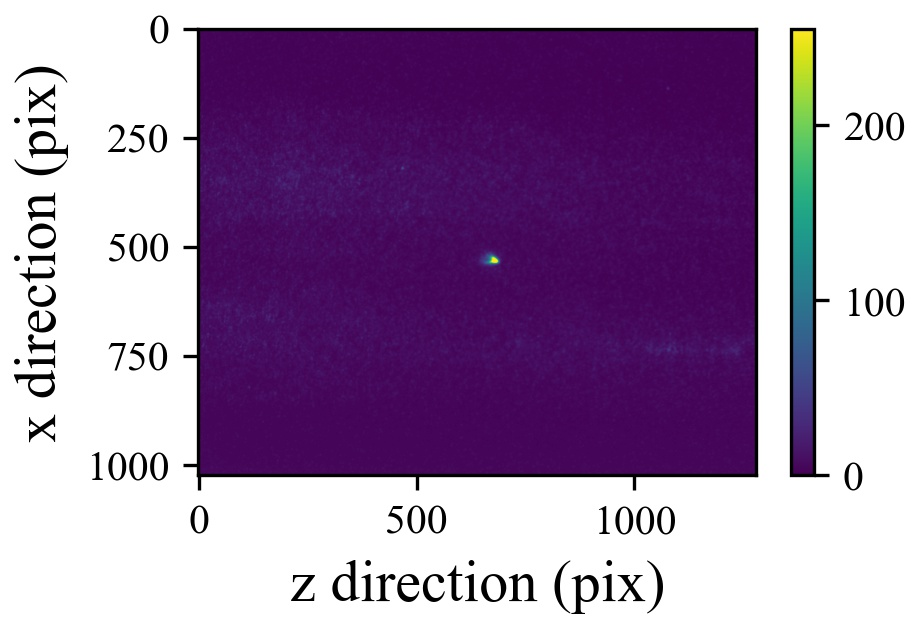
\includegraphics[width=0.98\columnwidth]{./theory/figure/5/image_0.jpg}
	\end{minipage}
	\begin{minipage}{0.3\linewidth}
		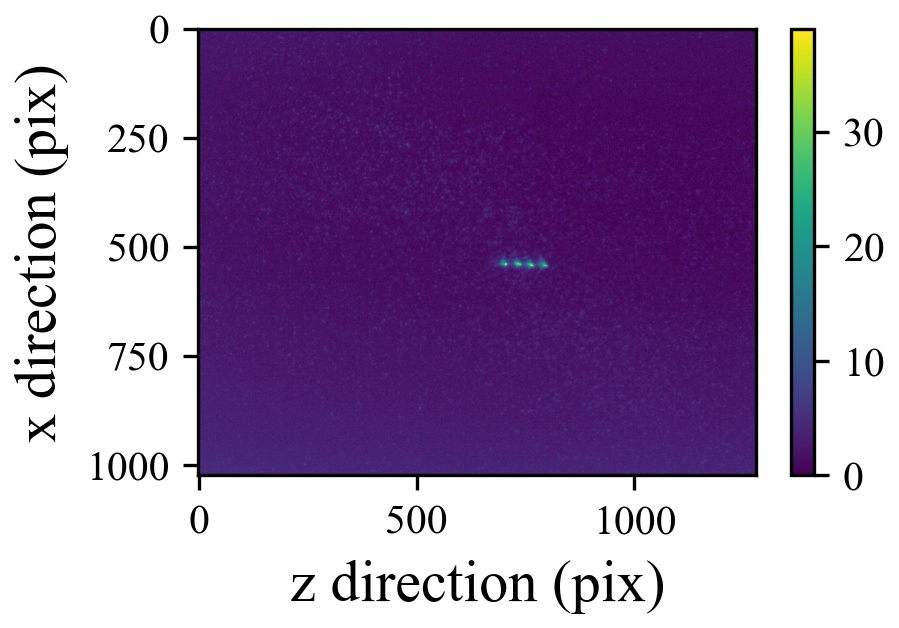
\includegraphics[width=0.98\columnwidth]{./theory/figure/5/image_1.jpg}
	\end{minipage}
	\begin{minipage}{0.3\linewidth}
		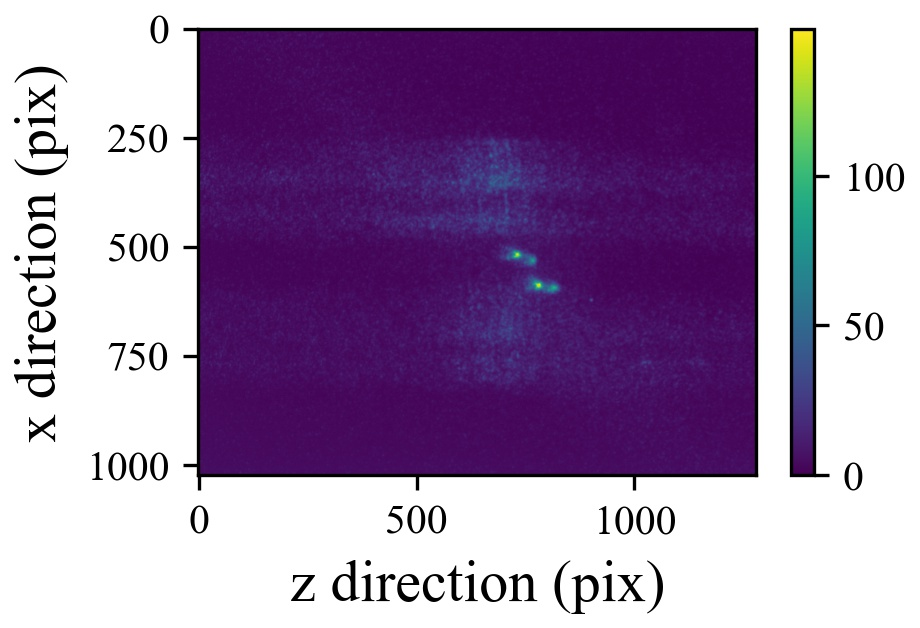
\includegraphics[width=0.98\columnwidth]{./theory/figure/5/image_2.jpg}
	\end{minipage}
	\end{center}
	\caption{集光系のピントおよびレーザー照射位置などが異なる場合のイオン捕獲画像}
	\label{fig:ionimage}
\end{figure}

\begin{figure}[h]
	\begin{center}
		\begin{minipage}{0.3\linewidth}
			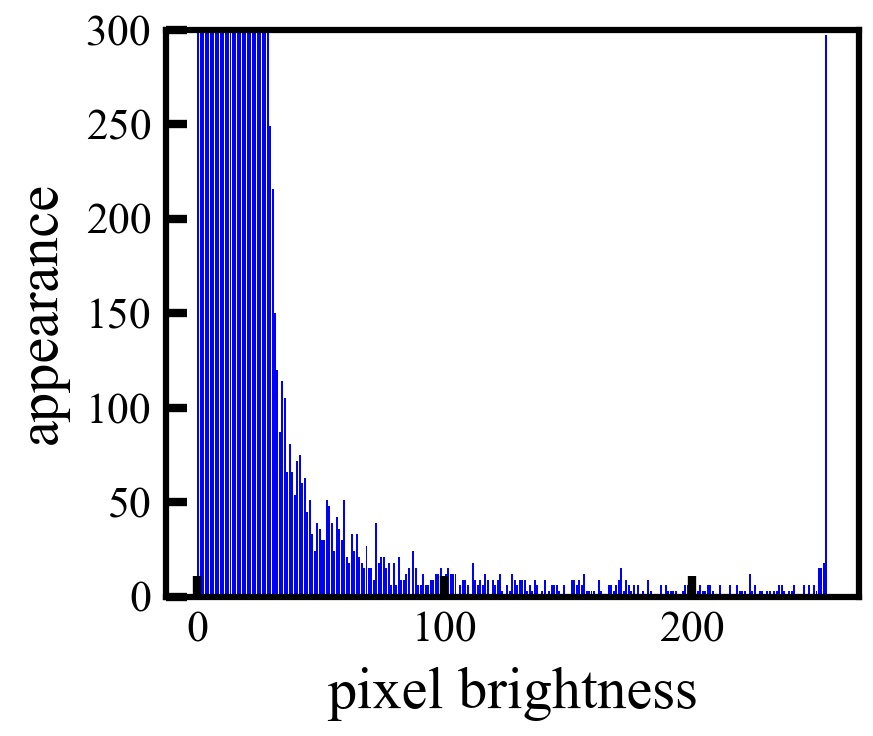
\includegraphics[width=0.98\columnwidth]{./theory/figure/5/hist_0.jpg}
		\end{minipage}
		\begin{minipage}{0.3\linewidth}
			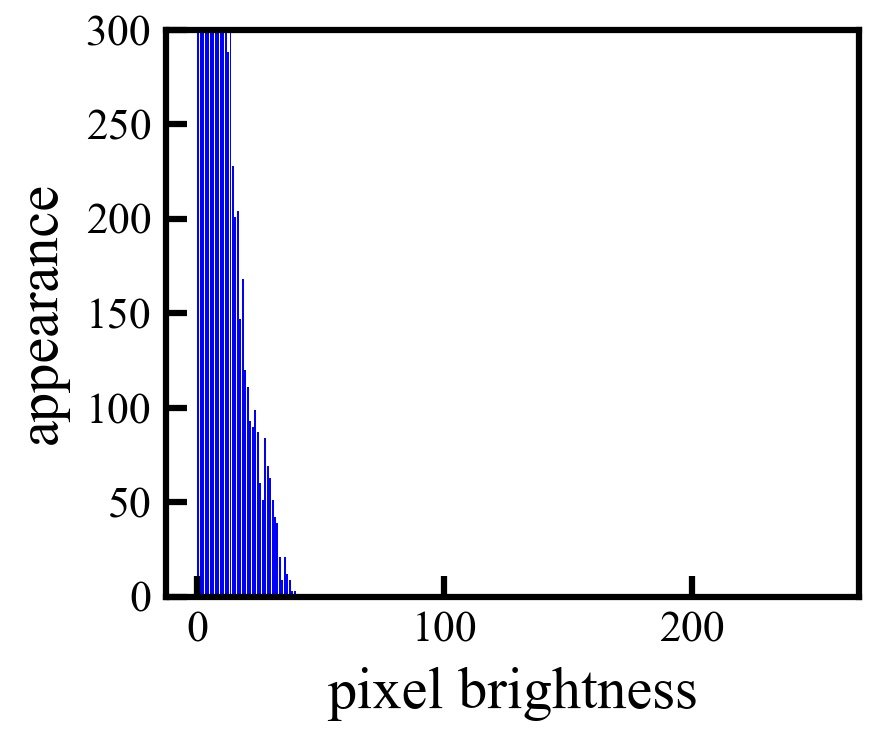
\includegraphics[width=0.98\columnwidth]{./theory/figure/5/hist_1.jpg}
		\end{minipage}
		\begin{minipage}{0.3\linewidth}
			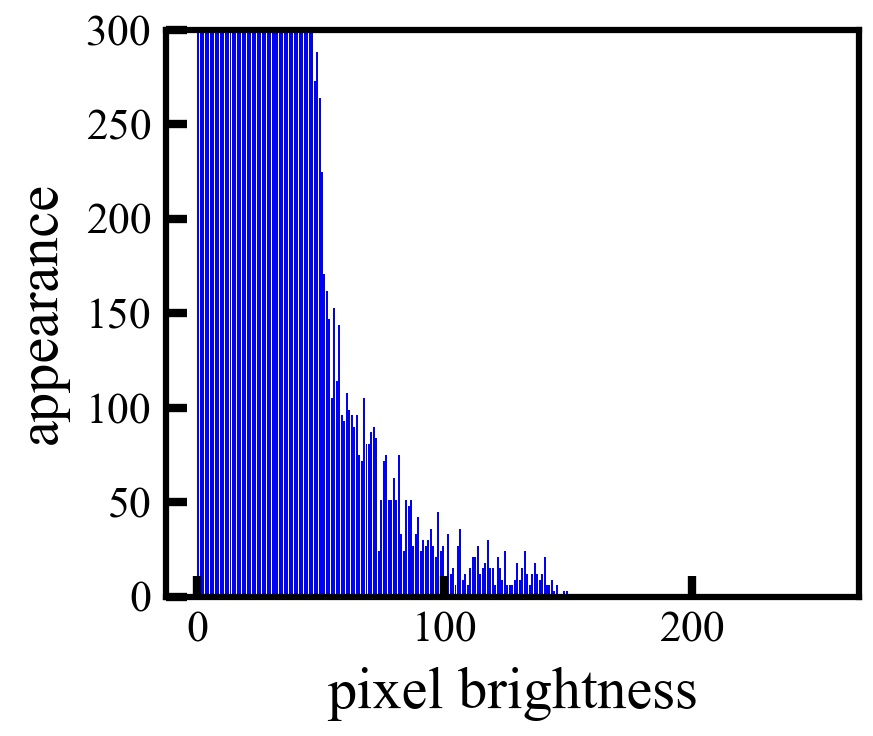
\includegraphics[width=0.98\columnwidth]{./theory/figure/5/hist_2.jpg}
		\end{minipage}
	\end{center}
	\caption{\Fig{ionimage}の各画像のピクセル輝度値のヒストグラム}
	\label{fig:hist}
\end{figure}

イオンの位置特定を行うに際し,二値化の処理のための閾値を定める.しかし,\Fig{hist}のように輝度値の偏りが各画像において異なっている場合,閾値を画像毎に変化させる必要がある.これを防ぐために濃度諧調変換と呼ばれるヒストグラムの正規化を行う.[c,d]の画素値を持つ画像を[a,b]のレンジに変換する式は次式で与えられる.

\large
\begin{align}\label{eq:GS_trans}
x_{\rm out} = 
\left\{ 
\begin{array}{ll}
	a & {\rm if} \ x_{\rm in} < c \\
	\frac{b-a}{d-c}(x_{\rm in}-c) + a & {\rm else \ if} \ c \leq x_{\rm in} < d \\
	b &{\rm else}
\end{array} \right.
\end{align}
\normalsize
ここでa,bは任意であり,cはある画像における輝度値の最小値,dは最大値とする.

\Fig{hist}に対して\Eq{GS_trans}を$a=0,b=255$として適用させると\Fig{norm_hist}となる.
\begin{figure}[h]
	\begin{center}
		\begin{minipage}{0.3\linewidth}
			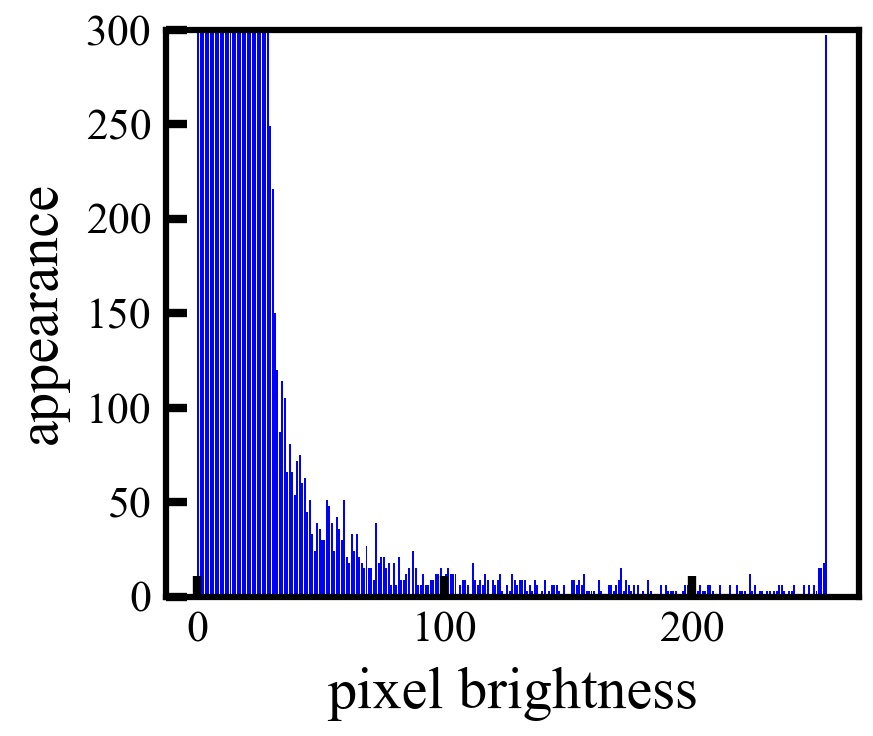
\includegraphics[width=0.98\columnwidth]{./theory/figure/5/norm_hist_0.jpg}
		\end{minipage}
		\begin{minipage}{0.3\linewidth}
			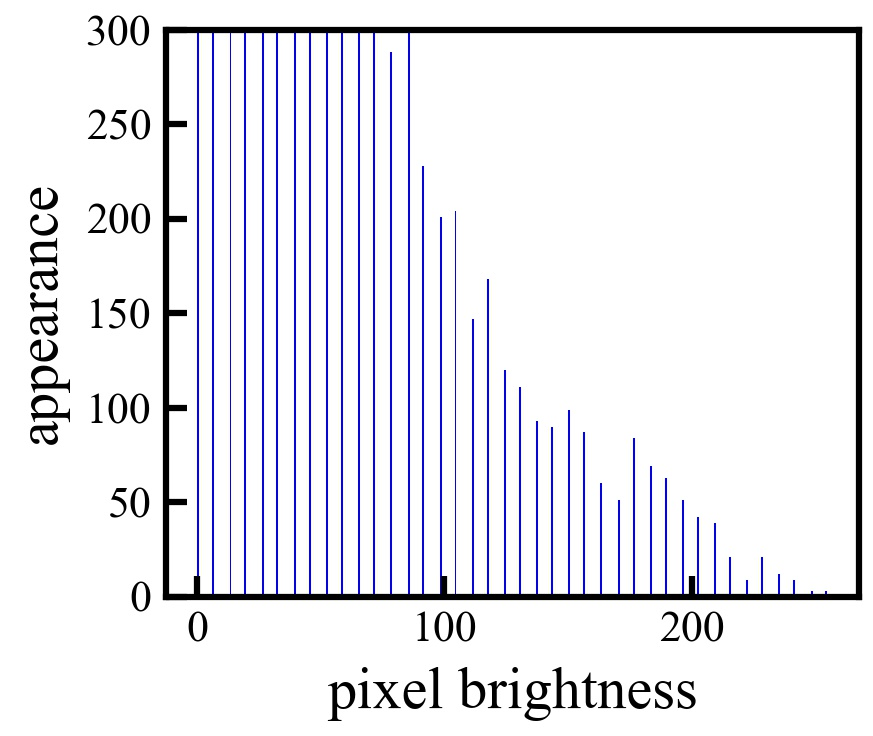
\includegraphics[width=0.98\columnwidth]{./theory/figure/5/norm_hist_1.jpg}
		\end{minipage}
		\begin{minipage}{0.3\linewidth}
			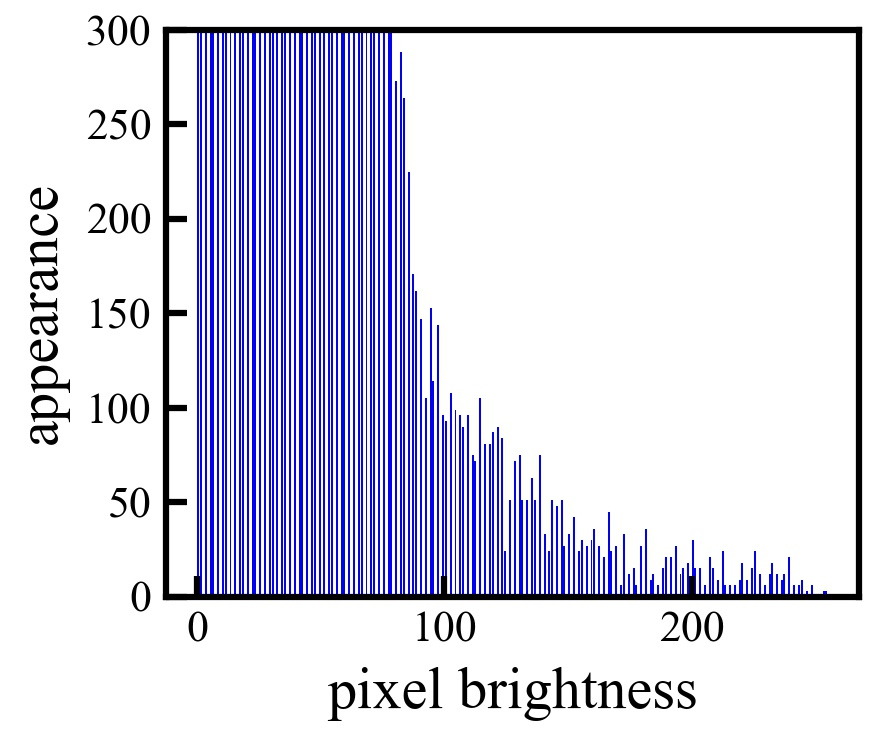
\includegraphics[width=0.98\columnwidth]{./theory/figure/5/norm_hist_2.jpg}
		\end{minipage}
	\end{center}
	\caption{\Fig{ionimage}の各画像のピクセル輝度値を正規化したときのヒストグラム}
	\label{fig:norm_hist}
\end{figure}

\subsection{二値化}
二値化とは,画像を特定の値を閾値として黒(=0)と白(=255)の2値で表現する方法である.二値化は次式で表される式を用いて変換される.
\large
\begin{align}\label{eq:binary_trans}
	x_{\rm out} = 
	\left\{ 
	\begin{array}{ll}
		0 & {\rm if} \ x_{\rm in} < {\rm threshold} \\
		255 & {\rm otherwise}
	\end{array} \right.
\end{align}
\normalsize
\Fig{thre_norm_hist}に\Eq{binary_trans}を${\rm threshold} = 128$として二値化を行ったときのヒストグラムを\Fig{binary_hist}に示す.
\begin{figure}[h]
	\begin{center}
		\begin{minipage}{0.3\linewidth}
			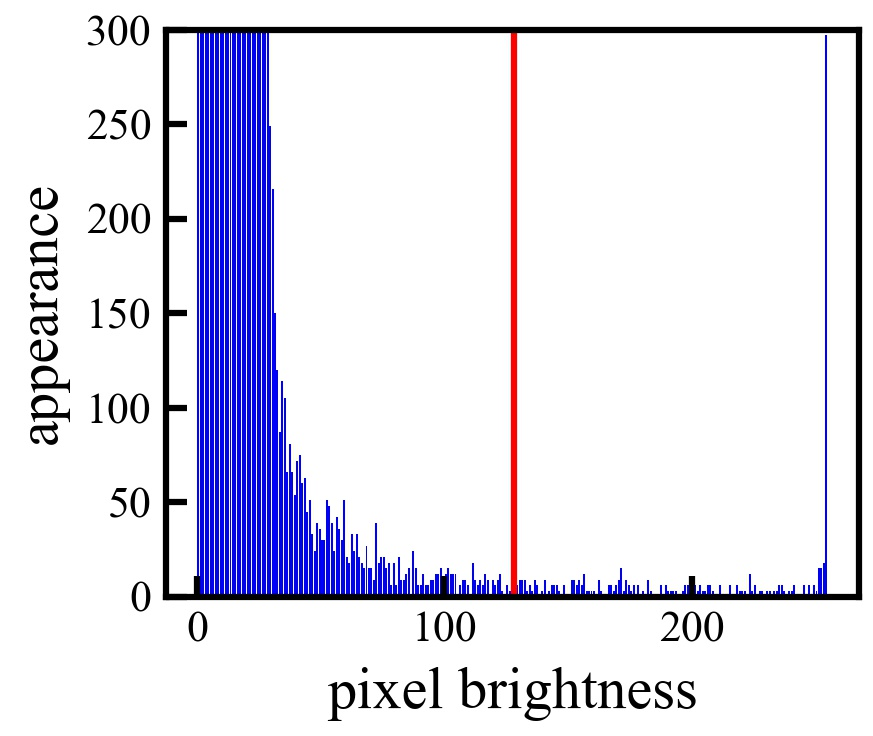
\includegraphics[width=0.98\columnwidth]{./theory/figure/5/thre_norm_hist_0.jpg}
		\end{minipage}
		\begin{minipage}{0.3\linewidth}
			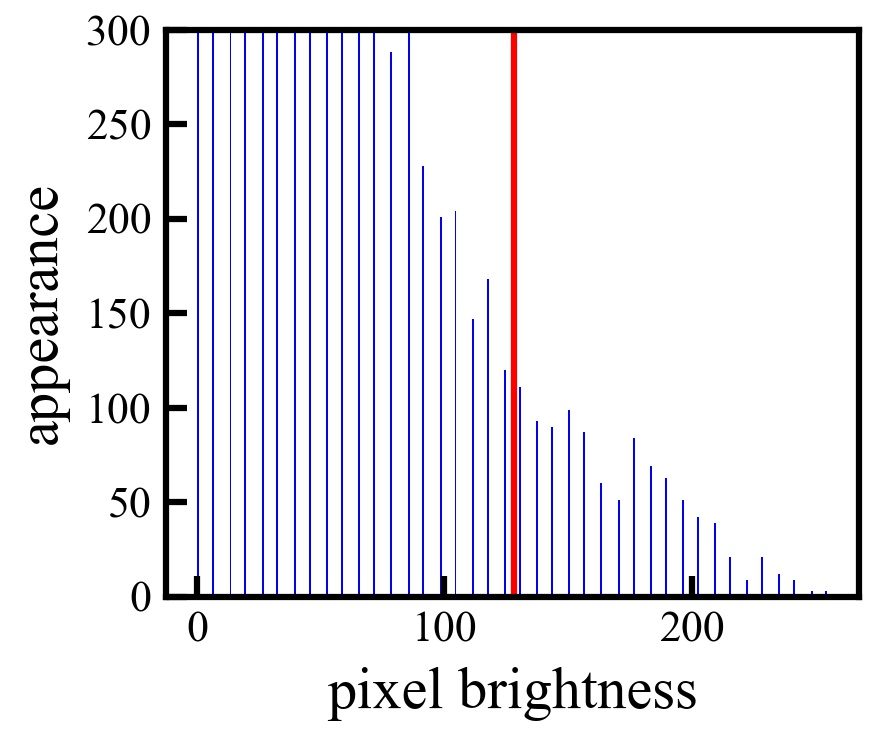
\includegraphics[width=0.98\columnwidth]{./theory/figure/5/thre_norm_hist_1.jpg}
		\end{minipage}
		\begin{minipage}{0.3\linewidth}
			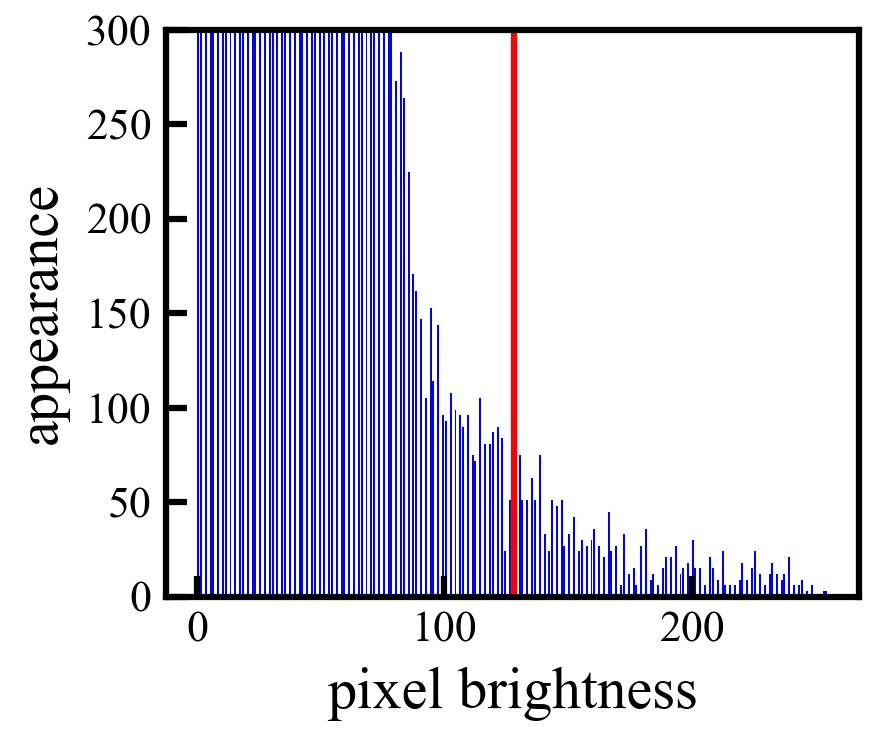
\includegraphics[width=0.98\columnwidth]{./theory/figure/5/thre_norm_hist_2.jpg}
		\end{minipage}
	\end{center}
	\caption{正規化されたヒストグラムにおける閾値(threshold = 128)の設定}
	\label{fig:thre_norm_hist}
\end{figure}

\begin{figure}[h]
	\begin{center}
		\begin{minipage}{0.3\linewidth}
			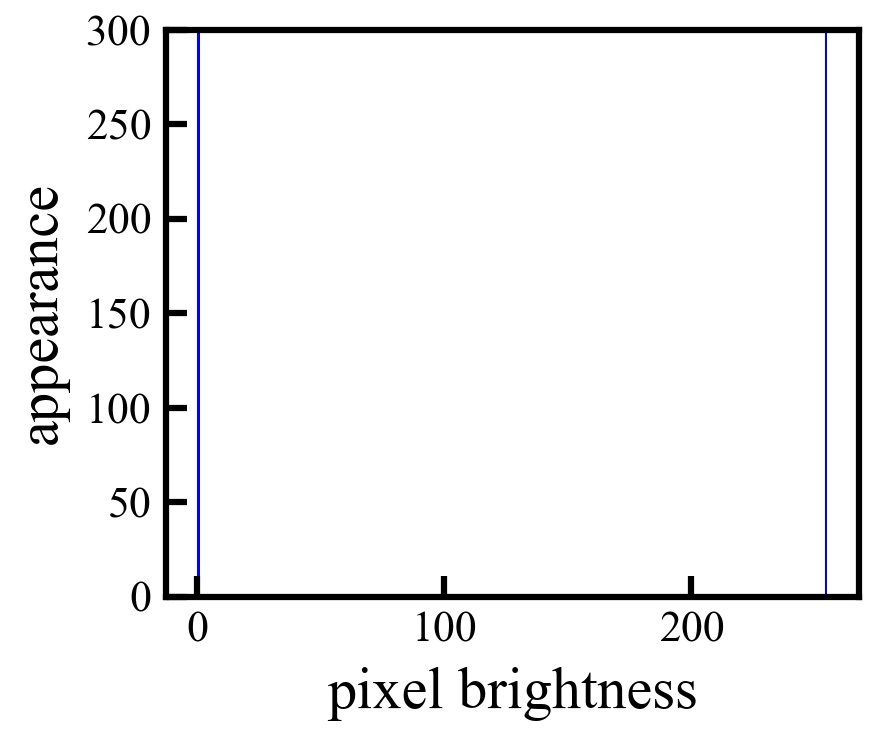
\includegraphics[width=0.98\columnwidth]{./theory/figure/5/binary_0.jpg}
		\end{minipage}
		\begin{minipage}{0.3\linewidth}
			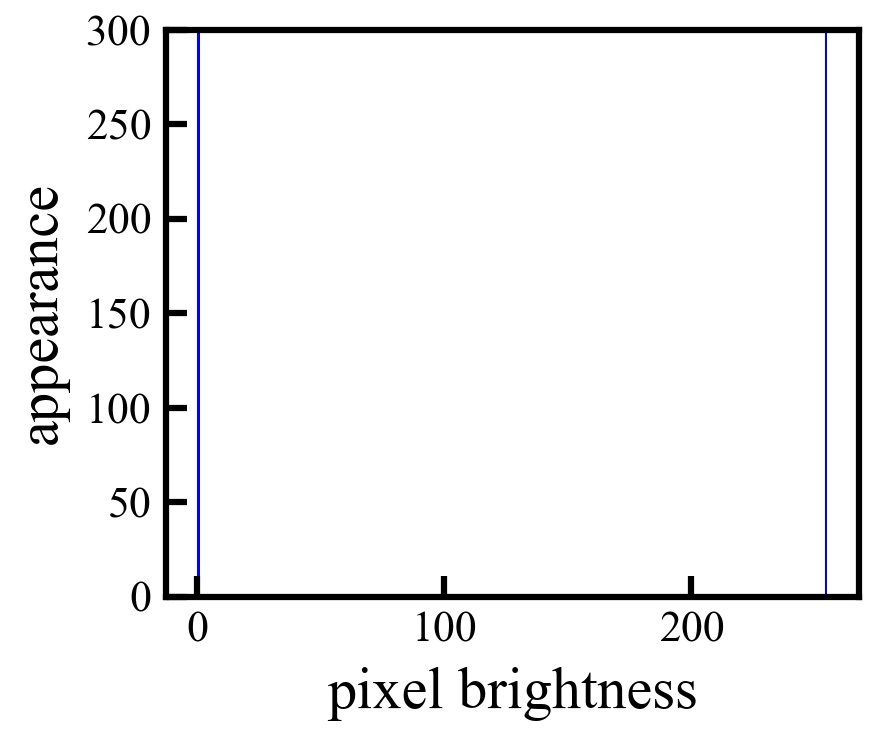
\includegraphics[width=0.98\columnwidth]{./theory/figure/5/binary_1.jpg}
		\end{minipage}
		\begin{minipage}{0.3\linewidth}
			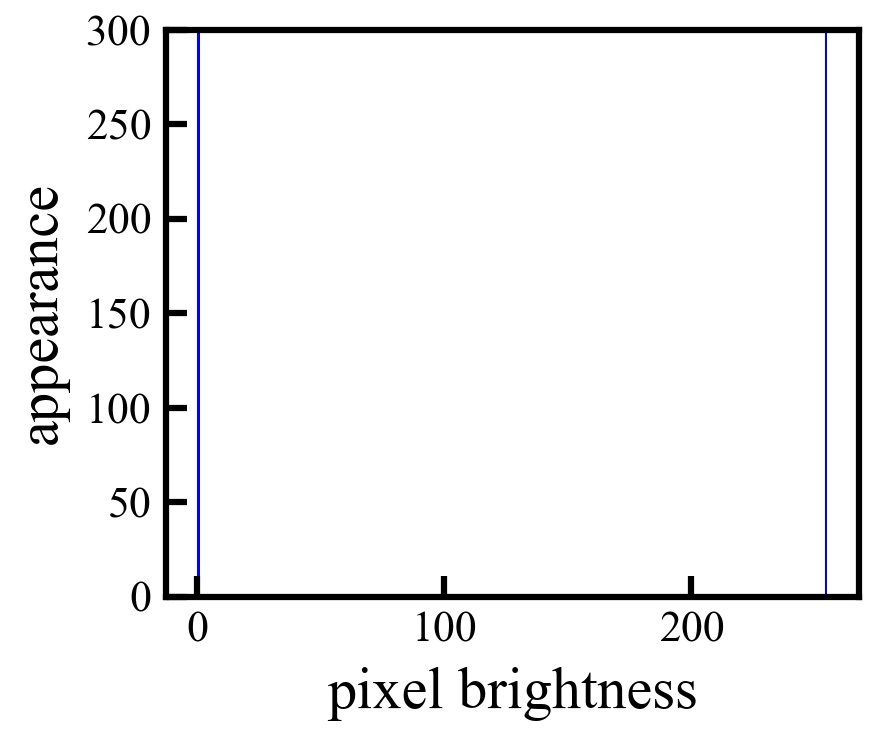
\includegraphics[width=0.98\columnwidth]{./theory/figure/5/binary_2.jpg}
		\end{minipage}
	\end{center}
	\caption{\Fig{thre_norm_hist}に対して,二値化(0,255)の処理を行った後のヒストグラム}
	\label{fig:binary_hist}
\end{figure}

ヒストグラムの正規化を行ったことで,カメラのピントや集光時間およびレーザーの波長や位置の影響を受ける画像の輝度値の二値化が固定の閾値で行うことができる.

\subsection{OpenCVを用いたイオンの検出}
二値化されたイオン捕獲画像において輝度値が255である範囲の面積を求め,ある値以上の面積を持つ範囲をイオンとして計上する.イオンと判定された範囲に対して最小外接円を近似しその中心値をイオンの位置として特定する.

\subsection{電場の算出方法}
イオンの位置を用いて,イオンにかかる電場の算出が可能である.N個のイオンが一列に並んでいるとき,i番目のイオンの座標$z_{i}$における電場$\bm{E}(z_{i})$を求める.イオンが捕獲されている状態では,プレーナートラップが形成する電場から受ける力と他のイオンから受けるクーロン相互作用による力とがつりあっている.したがって,次式が成り立つ.
\large
\begin{align}\label{eq:equi_string}
e\bm{E}(z_i) + \frac{e^2}{4\pi \varepsilon_0} \sum^N_{i=0,i\neq j} \frac{z_i - z_j}{|z_i - z_j|^3} = 0.
\end{align}
\normalsize
ここで,$e$は素電荷,$\varepsilon_0$は真空の誘電率を示す.
イオンが二列に並ぶ場合にも,\Eq{equi_string}と同様に平衡の式を満たす.i番目のイオンの位置が($z_i,x_i$)で指定されるとき,
\large
\begin{align}\label{eq:equi_array}
e\bm{E}(z_i,x_i) + \frac{e^2}{4\pi \varepsilon_0}\sum^N_{i=1,i\neq j}\frac{1}{|\bm{r}_{ij}|^2}\frac{\bm{r}_{ij}}{|\bm{r}_{ij}|} = 0,
\end{align}
\normalsize
と書くことができる.ここで,
\large
\begin{align}
\bm{r}_{ij} &= (z_i - z_j)\hat{z} + (x_i - x_j)\hat{x} \notag \\
|\bm{r}_{ij}| &= \sqrt{(z_i - z_j)^2 + (x_i - x_j)^2} \notag 
\end{align}
\normalsize
であり,$\hat{z},\hat{x}$は各軸における単位ベクトルである.また,$\hat{r}_{ij} \equiv \bm{r}_{ij}/|\bm{r}_{ij}|$とすれば,\Eq{equi_array}は,
\large
\begin{align}\label{eq:equi_array_2}
e\bm{E}(z_i,x_i) = \frac{e^2}{4\pi \varepsilon_0}\sum^N_{i=1,i\neq j} \frac{1}{|\bm{r}_{ij}|^2}\hat{r}_{ij} = 0
\end{align}
\normalsize
とまとめられる.二列配列のイオン捕獲位置における電場を導出する際には,\Eq{equi_array_2}を各軸に沿った成分毎に計算を行う.したがって,各成分に分けて書くと,
\large
\begin{align}
eE_z(z_i,x_i) + \frac{e^2}{4\pi \varepsilon_0} \sum^N_{i=1,i \neq j}\frac{z_i - z_j}{|\bm{r}_{ij}|^3} = 0 , \\
eE_x(z_i,x_i) + \frac{e^2}{4\pi \varepsilon_0} \sum^N_{i=1,i \neq j}\frac{x_i - x_j}{|\bm{r}_{ij}|^3} = 0 .
\end{align}
\normalsize
これを解くことで,
\large
\begin{align}
\bm{E}(z,x) = E_z(z,x)\hat{z} + E_x(z,x)\hat{x}
\end{align}
\normalsize
の関係から,イオン捕獲位置における電場の算出を行う.電場の大きさと,z軸からの偏角$\theta$は,
\large
\begin{align}
|\bm{E}(z_i,x_i)| &= \sqrt{E_z^2(z_i,x_i) + E_x^2(z_i,x_i)}, \\
\theta &= \tan^{-1} \left(\frac{E_x(z_i,x_i)}{E_z(z_i,x_i)} \right) .
\end{align}
\normalsize

\section{イオンの平衡位置}